
% Chapter Template

\chapter{Structure Depth Dataset}

\label{Chapter4:Dataset} 

%----------------------------------------------------------------------------------------
%----------------------------------------------------------------------------------------
%\url{https://fenix.tecnico.ulisboa.pt/downloadFile/1689244997256744/Thesis.pdf}

In this Chapter, we present our dataset created using Structure Sensor and we call it as \textbf{Structure Depth} dataset. The entire chapter is divided in to three sections. In the first section we discuss the technical details of the Structure Sensor and followed by the methods involved in creating this dataset. The last part of this chapter is about the various pre processing methods we used to performed for specific experimental setups.


\section{Structure Depth Dataset Overview} 

Our aim in this work is to deliver a robust system for depth prediction as seen in the Figure \ref{fig:Proposed_Model} for a portable hand held mobile device. In our case it is an IPad integrated with Structure sensor. In order minimize the difference between the predicted depth maps and depth map generated from Structure sensor we need to train with the similar dataset. We have also validated this in our experiments which will be discussed below in Section \ref{Chapter6:Results}. As discussed in the Section \ref{Chapeter1:Topic_Description}, this will also help us to study the effect of different camera and sensor properties on different environment.\\

As we have seen earlier in Chapter \ref{Chapter3:RelatedWork}, there are multiple datasets available but almost none fit our context. As we are already exploiting the depth features from NYU V2 for general prediction, we would like to produce a dataset which is solely application based. Here our application is mobile device, particularly IOS, we generate the dataset using an IPad. This will not only make the intrinsic parameters to be learned by the network but also particularize for IOS based devices. As we use IPad as integration, all the RGB Images are received from the IPad's camera. The features we want the neural network to learn and predict should have the same camera intrinsic parameters in order to decrease the amount of pre processing of the dataset. Hence, We first calibrate IPad with Structure Sensor before collecting the Dataset. Another major advantage of using Structure Sensor with an IPad over Kinect is the resolution of RGB and Depth Images. While Kinect V2 has $512\times424$ Infrared camera resolution, Structure Sensor can go upto $640\times480$. \\

Our Dataset consist of 2 versions. The first version(SD\_V1) which was taken during the training of \textbf{A1} network which is detailed in Section \ref{Chapter5:Methodology}. In V1, we produced no hole depth images with wall of threshold 4 m. Since the temporal resolution of Structure Sensor is as high as 60 fps, there is not much difference in frames. So, in order to achieve a quality dataset, we saved a frame in every 10\textsuperscript{th} frame. Having a 60 fps video stream, we saved 6 fps. This removes redundant data and prevents us from overfitting. In the second version(V2) of our dataset, we captured every 2\textsuperscript{nd} frame per second giving us a temporal resolution of 30 fps. In V2, we removed the distance threshold and filled it with holes instead. We trained \textbf{A2} network with the new dataset. Including V2, we have a total of 18 scenes and consisting of 2675 images captured using an Apple iPad Pro version 12.9 (2015) model and a Structure Sensor only. The dataset majorly includes images from office and classrooms environments. It consist of RGB Images of $640\times480$ as 3 channel $\times$ 8 bit int and Raw Depth Images of 640 $\times$ 480 as 1 channel. Both of the images are saved using lossless compression. Later, we also perform some processing to synchronize RGB and depth images and to fill the holes of depth image which will be discussed later in this chapter. We also provide the camera extrinsic parameters as a numpy matrix of $4\times4$ which is useful for reconstruction of a scenario.\\


\subsection{Technical Specification of Structure Sensor}
The Structure Sensor \footnote{\url{https://structure.io/}} is a 3D scanner introduced by Occipital in 2014. As the name suggests, it uses Structured-Light-System(SLS) 3D scanning\cite{Kalantari}. It can be easily attached to an IPad and with Structure SDK it enables us to generate good quality RGB image stream from IPad and its realtive depth stream from Structure Sensor at the simultaneously. As it only weighs 95 grams and can be used as an extension to mobile device, it makes the sensor very portable. With possibility of recording 60 frames per second at a resolution of $640\times480$\cite{Kalantari}. When compared to Kinect V2, it has more depth image resolution. The comparison can be seen in table \ref{table:KinectVsStructureSensor}. The minimum range it can capture is 40 cm while it can capture till 4 m with fine precision. After 4 m the precision is not satisfactory enough to use it for the dataset. Occipital claims it has low frame-to-frame noise and provides 100\% fill rate on most of the materials. On the other hand IPad Pro 12.9 provides us with an RGB video stream of $1920\times1080$ at 30 frames per second and $1080\times720$ at 60 frames per second. IPad Pro also provides us with Camera extrinsic parameters which are useful for the reconstruction of the scenario.\\

\begin{table}[h]
\begin{tabular}{@{}lll@{}}
\toprule
\textbf{Features}                    & \textbf{Kinect V2}           & \textbf{Structure Sensor}         \\ \midrule
Depth Sensor Type           & ToF & SLS                 \\
RGB Camera Resolution       & $1920\times1080$, 30 fps & $1920\times1080$, 60 fps     \\
IR Camera Resolution        & $512\times424$, 30 fps   & $640\times480$, 60 fps                 \\ 
Field of View of IR Camera  & $70^\circ\times60^\circ$           & $58^\circ\times45^\circ$                         \\
Recommended Operative Range & 0.4 m - 3.5 m       & 0.4 m - 3.5 m                                  \\
           &                     & 
\end{tabular}
\caption{Comparison of Kinect V2 and Structure Sensor}
\label{table:KinectVsStructureSensor}
\end{table}
\begin{figure}[h]
    \centering
    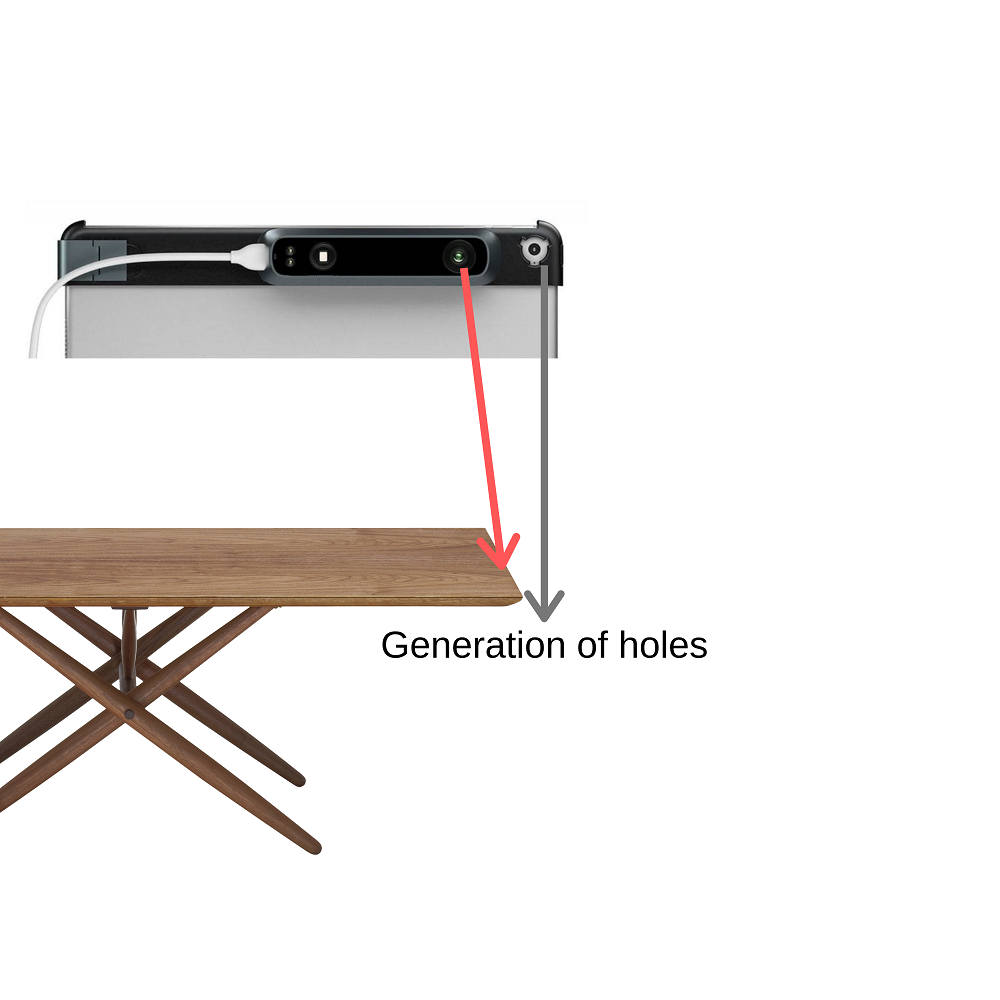
\includegraphics[scale=0.4]{Figures/holes.png}
    \caption{Generation of holes due to parallax}
    \label{fig:holes}
\end{figure}
While these sensors are great devices they have some limitations. The distance they can measure is limited and they suffer from reflection problems on transparent, shiny or very matte and absorbing objects. Another limitation is holes generated by parallax effect happening due to difference in position of the camera of IPad and Structure Sensor\cite{Kalantari}. In simpler terms, it works like human eyes. If we look at an object using only either of our eyes, we could notice disparities. When there is an object we try to focus on, our eyes which located at different position like the sensors in the Structure Sensor, they will see the object from different angles. If the object is close enough, then sometimes one eye can see what is behind and other can not. This can be seen in figure \ref{fig:holes}. As a result, it produces a shadow of holes which can be seen in figure \ref{fig:holes2}.



\begin{figure}[h]
    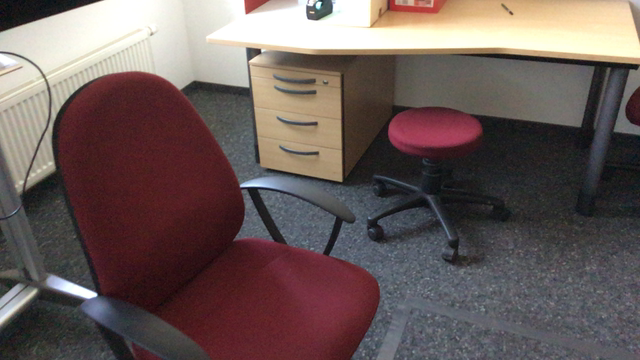
\includegraphics[scale=0.29]{Figures/RGB.png} 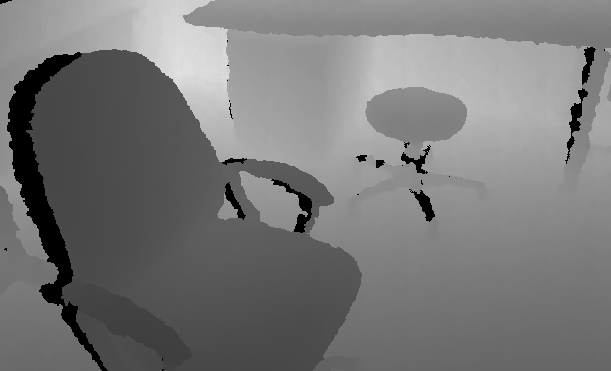
\includegraphics[scale=0.37]{Figures/Depth.png}
    \caption{Holes produced in depth image}
    \label{fig:holes2}
\end{figure}


\subsection{Dataset Collection}

A significant role in Machine Learning is played by Dataset and the collection of it makes most influence on the features that network learns. As the distance is limited in Structure Sensor and due to our scope of research we focus on indoor offices and classrooms environments. While capturing the dataset, one should keep in mind that the network should learn only the novel features not the artifacts. One good instance of this would be capturing the depth of a screen. Since, a screen has reflective black surface, it loses depth information resulting holes in depth image as seen in Figure \ref{fig:screens}. If we feed these images to the network, it might learn the features such as, screen is always at, let say x distance, where x is pixel value we assign to such holes. These holes are the undesired features and called artifacts. Such artifacts could be produced due to various reasons. It could be the reflective/absorbing nature of the surface of an object or the distance and position of the object\cite{geomar41830}. As a reflective/glossy surface leads us to wrong or no generation of depth pixel, we try to avoid them while capturing. Figure \ref{fig:screens} is one good example of such holes. As we notice in the RGB image there are two screens, one is predicted in some regions while other one is totally lost. In indoor environments, such objects are inevitable. Thus, in such problems we use techniques like inpainting \cite{inpainting}. Image inpainting could also be used to resolve artifacts due to parallax effect discussed in section previous section.\\
\begin{figure}[h]
    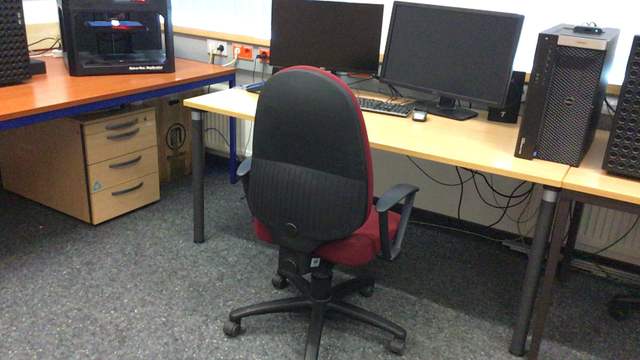
\includegraphics[scale=0.29]{Figures/7.png} 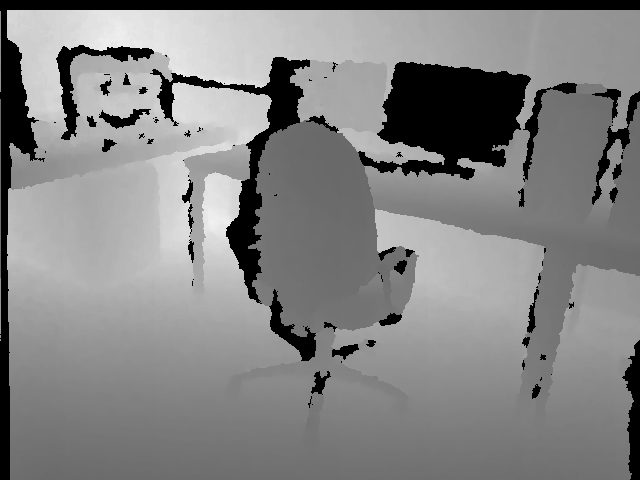
\includegraphics[scale=0.24]{Figures/Raw7.png}
    \caption{Holes produced in depth image due to reflectivity of the screen}
    \label{fig:screens}
\end{figure}
 

Since, the accuracy decreases with the increase in depth \cite{deptherror} and because the recommended range is no more than 4 metres(m) for Structure Sensor \cite{Kalantari}, we remove all the pixels which are far away than 4 m. These pixels can be resolved using further predictions and post processing. This also protects our network from learning the artifact of distant objects as a wall as discussed in \ref{Chapeter1:Topic_Description}.\\

\subsection{Data Processing}

The very first step of processing the dataset would be registering the depth pixels. After we have calibrated the camera, we convert the pixels received from Structure Sensor to millimetres(mm) for ease of understanding as the pixel value have a non linear relationship. After we have the distances in metres, we want to eliminate all the possible artifacts as these images still contain holes and precision less pixels. Usually, far away pixels have less precision and results in holes as well\cite{deptherror}. It is a good idea to conserve those pixels as holes in order to reconstruct the environment by later predicting the future frames. Firstly, after we have the Depth images in metres, we save all the holes by its pixel position or index for all the pixels more than 4000 mm so that we can use that information later. By doing so, we can eliminate the distance threshold artifact discussed earlier.

\begin{figure}[h]
    \centering
    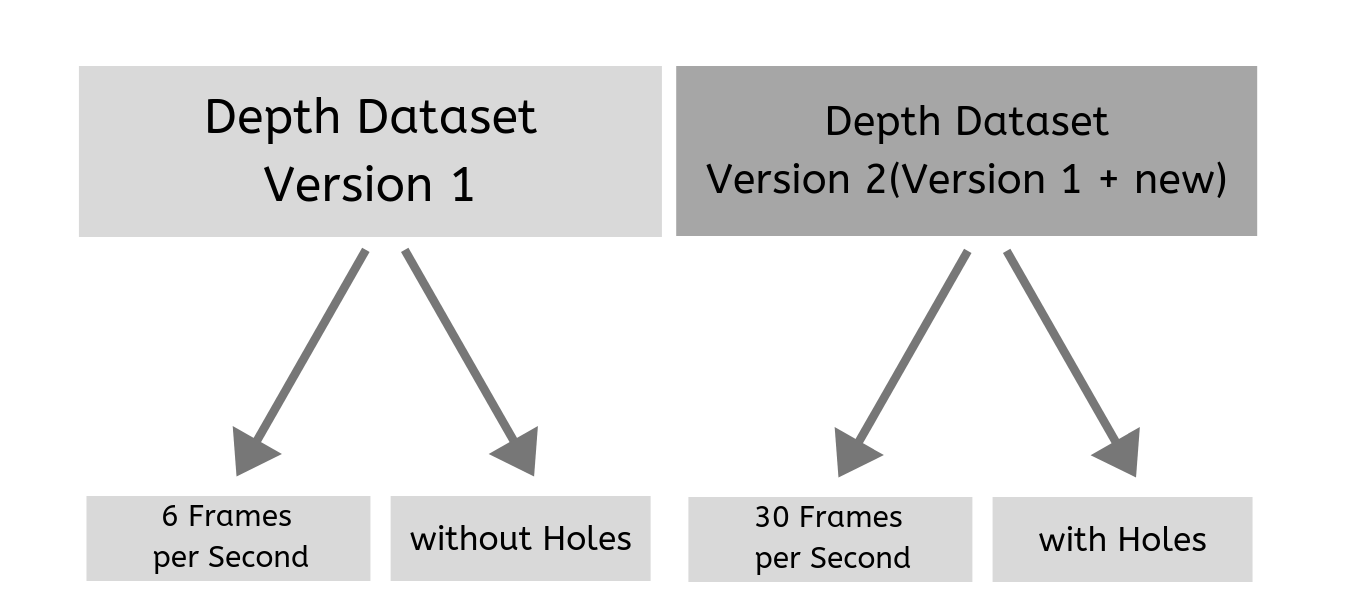
\includegraphics[scale=0.35]{Figures/versions.png}
    \caption{Versions of our proposed dataset}
    \label{fig:datasetversion}
\end{figure}

\begin{figure}[h]
    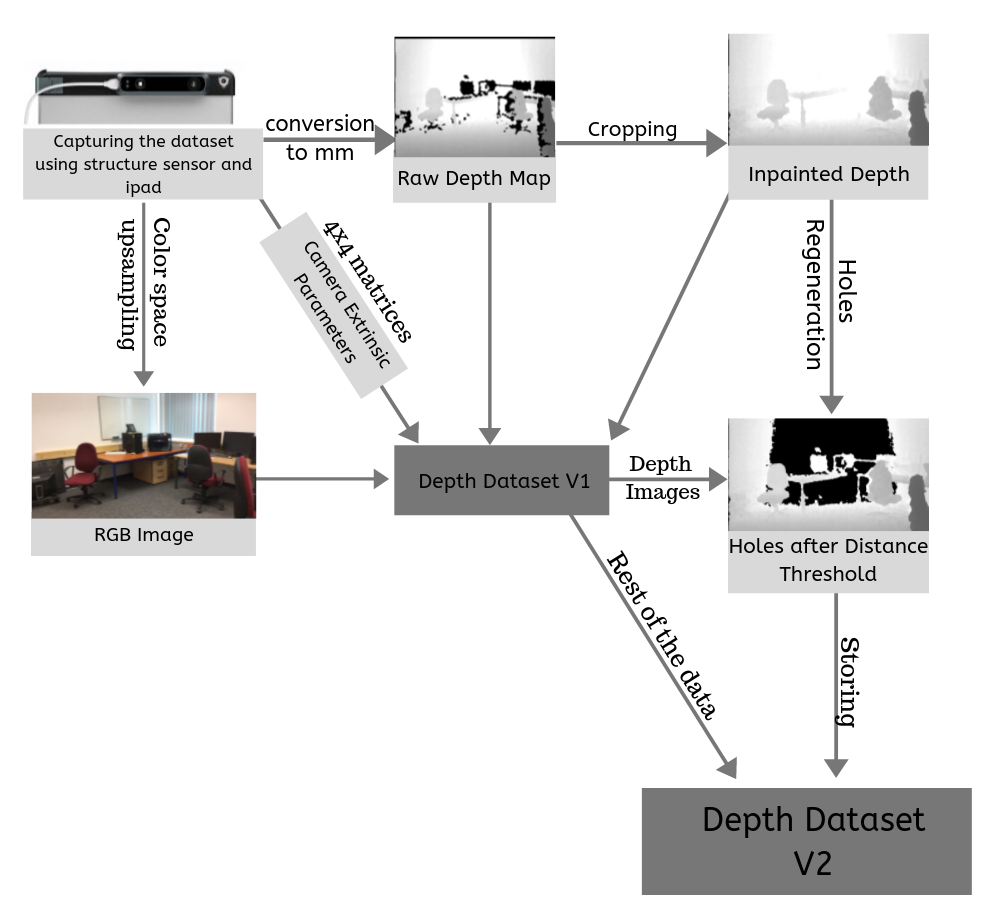
\includegraphics[scale=0.50]{Figures/process.png}
    \caption{Different stages of processing the depth frames}
    \label{fig:processing}
\end{figure}

As discussed earlier, the Depth images contains holes from shiny/glossy objects\cite{shiny}. In office environments, these holes are mostly generated by Computer Displays. Since we do not want our network to learn that all the screens are close(0 pixel), we interpolate these holes. We do this by inpainting \cite{inpainting} the whole image. This fixes the issues of shadows produced due to the parallax as well. Noting that it inpaints the pixels more than 4 m too. V1 of our dataset consisted of depth images which were totally inpainted and there were no holes as can be seen in \ref{fig:datasetversion}. Basically which means, if some of the pixels which are far away than 4 m are missing, they are interpolated using nearest neighbours. As we know, these predictions are not very accurate from past discussion, it is also possible that the inpainted depth is not correct. So In V2, successor of V1, we use the index of pixels of depth more than 4 m we saved now later in the process. This will reproduce all the holes which were more than 4 m as missing information is better than wrong predictions. These holes can later be predicted using the future frames. Our depth image is now ready to be fed to the network but as one would have noticed before, The size of the Color Image and Depth Image does not match since they have different aspect ratios due to different camera sources. So, In the end we crop the depth image centre focused in order to make them compatible with the network. We can understand this through Figure \ref{fig:processing}, where we show how the captured data and is processed and stored. \\






\newpage